\documentclass[conference]{IEEEtran}
\IEEEoverridecommandlockouts
% The preceding line is only needed to identify funding in the first footnote. If that is unneeded, please comment it out.
\usepackage{cite}
\usepackage{amsmath,amssymb,amsfonts}
\usepackage{algorithmic}
\usepackage{graphicx}
\usepackage{textcomp}
\usepackage{xcolor}
\usepackage{float}
\usepackage{subcaption}
\usepackage{graphicx}
\usepackage{tikz}
\usetikzlibrary{positioning}

\def\BibTeX{{\rm B\kern-.05em{\sc i\kern-.025em b}\kern-.08em
    T\kern-.1667em\lower.7ex\hbox{E}\kern-.125emX}}
\begin{document}

\title{Software Defined Radio Channel emulator GNSS\\ \large{\textit{Initial report}}}

\author{\IEEEauthorblockN{George Burns}
\IEEEauthorblockA{\textit{dept. Electrical and Electronic Engineering} \\
\textit{University of Bristol}\\
Bristol, United Kingdom \\
george.burns.2001@bristol.ac.uk}
}

\maketitle
\begin{abstract}
This report will detail proposed methods to simulate radio frequency (RF) wave propagation in the L-Band frequency range. It will detail the standards and mathematical models used to simulate some off the effects of on the propagation of RF waves from a satellite in orbit around the Earth to a ground station on Earth. There will also be detail on the modulation schemes used to test such simulation methods.
\end{abstract}

\section{Introduction}
In this section there will be a list of the effects that will be detailed in this report and simulated in the Channel Emulator. Satellite communications come under attenuation both complex and real \cite{seybold_introduction_2005}. Most channel emulators for these effects are expensive and hard to implement however the aim of this projects is to construct software that simulates these effects.\\

Using \cite{seybold_introduction_2005} as a basic reference point a basic model can be constructed. As shown in Figure \ref{fig:System_model}. 
\begin{figure}[h]
\centering
	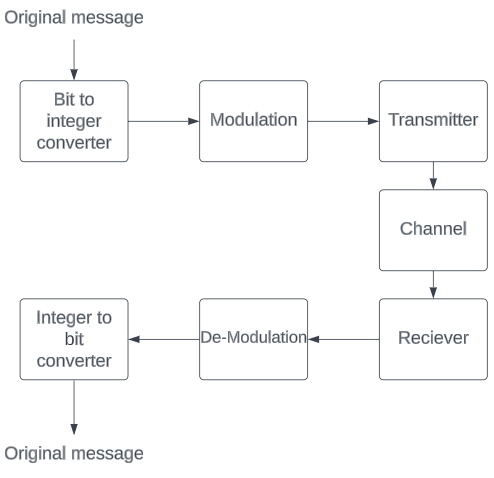
\includegraphics[width = 0.45\textwidth]{System_model.png}
	\caption{Full System Model}
	\label{fig:System_model}
\end{figure}

The Majority of the work will be focused on the Channel Emulator part of the system.\\

The Emulator will primarily focus on the following effects; Free space loss, Atmospheric Effects, Rain Fade, Noise Temperature, multipath fading and scintillation and the effects of orbit. All of these effects have a significant impact on the channel \cite{kaplan_understanding_2017}. Effects like multipath and sun outages are not being considered in this project as they are beyond the scope and are highly area and condition dependent. All the effects stated previously are both complex and real impairment. This means that for an electromagnetic wave represented as $Ae^{j w t+\theta}$, the channel will impair the amplitude ($A$), the phase ($\theta$), and the frequency ($w = 2\pi f$), where $f$ is the frequency and $j= \sqrt{-1}$ is the imaginary number. These effects where chosen in accordance with \cite{kaplan_understanding_2017} which details these effects as being prominent in GNSS systems.\\

These effects are also dependent on time as during the orbital period of the satellite both slant angle \cite{seybold_introduction_2005} and the distance can also change \cite{10.5555/2601574}, these effects will be detailed in section \ref{sec:Orbital}). Effects like ionospheric effects and rain attenuation are also dependent on time and location as well as weather conditions.
\label{sec:intro}


\section{Modulation TOO BE REVISED}
GNSS systems use binary phase shift keying (BPSK) to generate the bit sequence required to transmit the information. In conjunction with direct sequence spread spectrum (DSSS) that generates a pseudo-random code that involves "inserting" a code into the original signal to prevent jamming. In the scope of this project there will simply be an implementation of BPSK as the the interest is the effect of the channel on this signal rather then the effect of the generation/ implementation of the pseudo-random nature of the signal. Shown below is a constellation diagram of a BPSK signal in figure X.\\

To explore the atmospheric and other effects I have also developed both multi array frequency shift keying (MFSK) and multi array amplitude key shifting (MASK). These modulation schemes will give a valuable insight into the effects of the channel. 
\label{sec:Modulation}


\section{Free Space loss}
Equation \ref{eq:Free_space_equation} is used to model free space loss. Free space loss is the natural loss that occurs between all RF communication links \cite{seybold_introduction_2005} however for Earth to space extra factors need to be considered. On the terrestrial plane $r_s$ is usually just distance between two terrestrial links however slant path needs to be accounted for in space-Earth paths. $r_s$ can be calculated using Equation \ref{eq:Slant_path_equation} and is shown in Figure \ref{fig:Slant_path_illustration}\\
\begin{equation}
A_{fs} = \frac{(4 \pi r_s)^2}{\lambda^2 }
\label{eq:Free_space_equation}
\end{equation}

Where $A_{fs}$ is free space loss, $A_r$ and $A_t$ are the area of transmitter and receiver antenna respectively $\lambda$ is wavelength and $r_s$ is slant path.\\
\begin{figure}[h]
\centering
	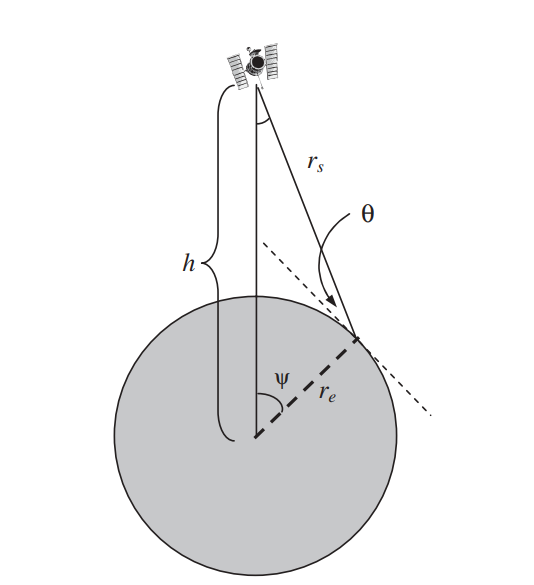
\includegraphics[width = 0.45\textwidth]{Slant_path.png}
	\caption{Slant Path illustration from \cite{seybold_introduction_2005}}
	\label{fig:Slant_path_illustration}
\end{figure}


\begin{equation}
r_s = \frac{h sin(\psi)}{sin(\frac{\pi}{2}+\theta)}
\label{eq:Slant_path_equation}
\end{equation}

Where $h$ is the height above Earth, $r_e$ is Earth's radius $6378K m$, $\theta$ is the elevation angle and $\psi$ is the central angle determined by equation \ref{eq:Central_angle_equation}.\\

Thus as the satellite changes distance (slant path $r_s$), the free space attenuation changes. Also Doppler effects cause frequency changes and thus wavelength ($\lambda$) changes, this is explained more in \ref{sec:Doppler}.  

\begin{equation}
\psi = cos^{-1}(\frac{r_e}{h}(sin(\frac{\pi}{2}+\theta))-\theta
\label{eq:Central_angle_equation}
\end{equation}

\label{sec:Free_space}

\section{Atmospheric Attenuation}
Effects of the atmosphere along the slant path $r_s$ must be considered when modelling RF propagation through Earth's atmosphere, its effects can be mathematically modelled as having distinct layers. The full mathematical model is complex so the goal was to use the International Telecommunications Union's (ITU) curve fitting process. Using \cite{ITU-R_P.676-5} to gain $\gamma_{o}$ the oxygen attenuation and $\gamma_w$ the water attenuation we can get an expression for atmospheric attenuation from \cite{ITU-R_P.618-7} to form equation \ref{eq:Atmospheric_attenuation_equation}.
\begin{equation}
A_a = \frac{h_o \gamma_o + h_w \gamma_w}{sin(\theta)}
\label{eq:Atmospheric_attenuation_equation}
\end{equation}
Where $A_a$ is the atmosphere attenuation in $dB$, $h_0$ is the oxygen height and $h_w$ is the water vapour height both obtained by using the curve fit equation found in \cite{ITU-R_P.618-7}.

\label{sec:Atmosphere}

\section{Rain Attenuation}
Hydrometeors are small water particles in the atmosphere can cause RF attenuation and thus must be accounted for in the model ITU provides a suitable model where \cite{ITU-R_P.837-1} provides the $R_{0.001}$ rain statistic which is the $0.01\%$ rainfall rate for the specified latitude and longitude. Then in conjunction with \cite{ITU-R_P.618-7} we can develop the rain model necessary. This factor is dependent on frequency, pressure, temperature, surface height of the antenna and many other factors. The final output produces a overall probability of a certain $dB$.\\

\label{sec:Rain}


\section{Scintillation}
Scintillation can both be accounted for using ITU recommendations in \cite{ITU-R_P.618-7} both for $\theta> 5°$ and $\theta < 5°$. These are all dependent on location and measurements from that area for parameters such as average humidity and temperature. For frequencies below $10G Hz$ Scintillation is more prevalent in the ionosphere and can be accounted for using models present in \cite{ITU-R_P.531-14}.\\ 

Scintillation in the troposphere can also again be modelled by \cite{ITU-R_P.618-7} and is more relevant to this projects as it details the scintillation prevalent in the troposphere at $f > 1G Hz$. Thus this mathematical model will be used to model scintillation.


\label{sec:Scintillation}

\section{Noise temperature}
The noise equation (equation \ref{:eq:Noise_equation}) states that noise is directly proportional to temperature. 
\begin{equation}
N = kT
\label{:eq:Noise_equation}
\end{equation}
Where $N$ is noise, $k$ is Boltzman's constant and $T[K]$ is temperature in Kelvin\\

Temperature can effected by a large array of systems and are detailed further in \cite{ITU-R_P.372-16}. The model I choose to implement is from \cite{ITU-R_P.618-7} and shown in equation \ref{eq:Noise_temp_equation}
\begin{equation}
T_s = T_m(1-10^{-A/10})
\label{eq:Noise_temp_equation}
\end{equation}
Where $T_s[K]$ is the temperature seen at the antenna in kelvin, $A[dB]$ is path attenuation found in both \ref{sec:Free_space} and \ref{sec:Atmosphere} and $T_m [K]$ is the effective temperature in Kelvin.\\

Thus substituting $T_s$ in \ref{eq:Noise_temp_equation} with $T$ in \ref{:eq:Noise_equation} we can find a suitable value for noise in the system. This is relevant as $T_s$ is highly dependent on atmosphere temperature. 

\label{sec:Noise_temp}


\section{Doppler effect}
When an object is moving at high speeds it experiences the Doppler effect. To model this equation \ref{eq:Doppler_effect_equation} can be used. 
\begin{equation}
f_{new} =(\frac{v_d+c}{v_s+c})f
\label{eq:Doppler_effect_equation}
\end{equation}
Where $f_{new}$ is the perceived frequency of the RF wave, $v_s$ is the speed of RF source, $v_d$ is the speed of receiver, $c$ is the speed of light in the medium and $f$ is the original frequency.\\

This equation is significant as the majority of the effects covered previously depend on the perceived frequency $f_{new}$. This effect is extremely prevalent on systems where the speed of the source (satellite) is not constant during the orbital window as this can mean a frequency change during the pass and thus the de-coding system is time dependent thus this aspect of the project is extremely important. This effect causes a "s" curve effect to occur shown in figure \ref{fig:Doppler}.

\begin{figure}[h]
\centering
	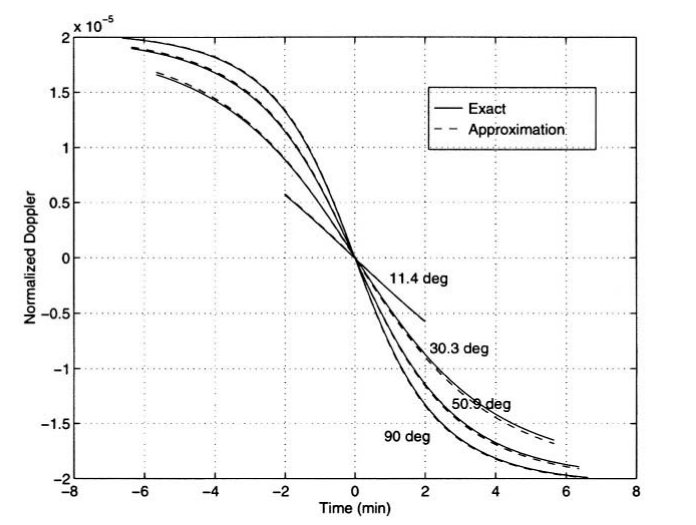
\includegraphics[width = 0.45\textwidth]{Doppler_s_curve.png}
	\caption{Actual and approximate Doppler S-curve for different maximum elevation angles from \cite{doppler_effect}}
	\label{fig:Doppler}
\end{figure}

\label{sec:Doppler}

\section{Orbital considerations}
In previous sections particular attention has been paid to slant path $r_s$ this is especially important when considering satellite systems with elliptical orbits as the slant range is not constant for the orbital period. This no doubt changes a large amount of parameters outlines previously and the system becomes highly dynamic thus all previously mentioned sources of channel degradation change significantly during the orbital period of satellite.\\

All this can be calculated using an orbital propagator like SGP4 that takes two line element (TLE) inputs and returns the height of the satellite that can then be used to find the slant height from \ref{eq:Slant_path_equation} and inclination is directly obtained from the TLE. TLE's are orbital parameters that are transmitted from the satellite periodically and there layout is shown in figure \ref{fig:TLE}.

\begin{figure}[h]
\centering
	\includegraphics[width = 0.45\textwidth]{TLE.png}
	\caption{TLE diagram from \cite{TLE_flat_earth}}
	\label{fig:TLE}
\end{figure}

For example a GPS satellite that has a speed of $14000 Km/s$ and transmitting a signal at $1G Hz$ we can calculate the perceived frequency using \ref{eq:Doppler_effect_equation} and $v_d$ is zero as the speed of that station is zero relative to the Earth's reference frame.\\

\begin{equation}
\centering
\begin{split}
f_{new} =& (\frac{v_d+c}{v_s+c}) f\\
\therefore f_{new} =& (\frac{c}{v_s+c})f\\
\therefore f_{new} = &(\frac{3\cdot 10^8}{14000 \cdot 3\cdot10^8}) 1\cdot 10^9\\
\therefore f_{new} =& 0.714\cdot  10^9
\end{split}
\label{eq:Doppler_example}
\end{equation}

\label{sec:Orbital}
\bibliographystyle{IEEEtran}
\bibliography{My_Library}
\end{document}
